\documentclass[titlepage]{article}
\usepackage{graphicx,tikz, float}
\usepackage{hyperref}
\usepackage{listings}
\usepackage{xcolor}
\lstdefinestyle{sharpc}{language=[Sharp]C,
frame=lr}
\title{Comparative Programming Languages: Assignment 2:\\Domain Specific
Language}
\lstset{style=sharpc, frame=L}
\author{Willem Van Onsem\\Jonas Vanthornhout\\Pieter-Jan Vuylsteke}
\date{January 11, 2013}
\newcommand{\Csh}[0]{\texttt{C\#} }
\newcommand{\itembf}[1]{\item \textbf{#1}: }
\newcommand{\itemit}[1]{\item \textit{#1}: }
\newcounter{ucc}\setcounter{ucc}{1}
\newcommand{\ucdef}[8]{\subsection{\emph{UC\arabic{ucc}}:
#1}
\begin{itemize}
 \if\relax\detokenize{#1}\relax\else
 \itembf{Name}#1
 \fi\if\relax\detokenize{#2}\relax\else
 \itembf{Primary actor}#2
 \fi\if\relax\detokenize{#3}\relax\else
  \itembf{Secondary actor}#3
 \fi\if\relax\detokenize{#4}\relax\else
   \itembf{Interested parties}\begin{itemize}#4\end{itemize}
 \fi\if\relax\detokenize{#5}\relax\else
 \itembf{Preconditions}\begin{itemize}#5\end{itemize}
 \fi\if\relax\detokenize{#6}\relax\else
 \itembf{Postconditions}\begin{itemize}#6\end{itemize}
 \fi\if\relax\detokenize{#7}\relax\else
 \itembf{Main scenario}\begin{enumerate}#7\end{enumerate}
 \fi\if\relax\detokenize{#8}\relax\else
  \itembf{Alterantive scenarios}\begin{enumerate}#8\end{enumerate}
 \fi
\end{itemize}
\addtocounter{ucc}{1}}

\begin{document}
\begin{titlepage}
\maketitle
\end{titlepage}
\tableofcontents
\newpage
\section{Domain description and analysis}
In the domain model below, the elements in our domain are shown.
\begin{figure}[H]
	\centering
	\includegraphics[scale=0.60]{../../../Domeinmodel/Domeinmodel.png}
	\caption{Het domeinmodel}
	\label{cd:domeinmodel}
\end{figure}

\section{Design description}
\subsection{The semantic model}
\subsection{DSL constructs}

% !TEX root = dslreport.tex

\section{Implementation overview}
Our DSL isn't really based upon an API. We've implemented our own compiler, this is explained in subsubsection \ref{sssection:motivation_for_the_compiler}. Of course in order to execute the programs written in the DSL we need some communication with the database. This is done with the library \texttt{Npgsql} and more in detail the classes \texttt{IDbConnection} and \texttt{IDbCommand}. However our usage of this API is a very primitive, we only need to open, close and execute queries on the database. When we need to transform data from the database to the objects from the database frontend, we need a system that provides this operations in its API. This is done with the class \texttt{IDataReader} which provides operations such as \texttt{GetString}, \texttt{GetInt32}, ... these methods transform the data of the cell into the desired type. Another interesting method is \texttt{GetOrdinal}, this method returns the position of the column with the given name. This way we can extract information from the database.
% !TEX root = dslreport.tex

\subsection{Justification of the chosen language}
We have chosen to use the language C\# for this project. Because we wanted to make a graphical DSL, we needed a language that is suitable for making graphical applications. Above that, we needed to work with a database. The C\# language is well suited for this. Only one of us knew the language well, so a good knowledge of the chosen language wasn't a reason for choosing this language.

\section{DSL implementation}
The system basically consists out of three parts: a user interface front-end, 
a database back-end and an adapter layer between them. The frontend can ask to 
execute a query on the database. Then, the appropriate adapter class can make this 
request suitable for the database back-end. It is important to note that
the user-interface only checks for language consistency. For instance it checks
if the primitives are ordered appropriately, but it doesn't check for instance if
a certain country actually exists in the database. The back-end assumes the
entered intermediate code is consistent and only executes the queries. Both
parts are written in \Csh{}. The database part invokes a \texttt{PostgreSQL}
database. Figure \ref{fig:systemOverview} gives a graphical overview of the system.
\begin{figure}[hbt]
\centering
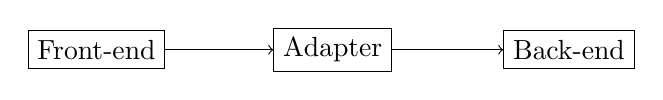
\begin{tikzpicture}
\node[rectangle,draw=black] (F) at (-3,0) {Front-end};
\node[rectangle,draw=black] (A) at (0,0) {Adapter};
\node[rectangle,draw=black] (B) at (3,0) {Back-end};
\draw[->] (F) to node[below]{} (A);
\draw[->] (A) to node[below]{} (B);
\end{tikzpicture}
\caption{Graphical overview of the System}
\label{fig:systemOverview}
\end{figure}
\paragraph{}We will describe each of the parts in detail in the sections below. The code can be found in the directory \texttt{DSLImplementation}.
% !TEX root = dslreport.tex

\subsection{User interface}
\subsubsection{Overview}
The user interface describes the way how the user will communicate with the
system, and thus by extend contains the domain specific language. In our case
we've implemented a graphical language. Furthermore we've implemented a fully
modifiable two-stage compiler.
\subsubsection{Motivation for the graphical language}
Since most users who will use the systems are end-users and thus not
programmers or technical people, some problems might occur with textual
languages. Most end-users nowadays don't use any command line tools anymore and
have no proper understanding of technical textual languages. By implementing a
graphical language, we aim to solve the following problems:
\begin{itemize}
 \itemit{A more semantical granularity} a problem with textual languages is
the granularity, namely the character. Characters don't map to concepts
directly. With graphical languages, we can foresee a primitive for each concept
in the language. Therefore people have a better understanding of their queries.
Furthermore one can easier debug aspects (since there are less issues with
writing an incorrect character sequence).
 \itemit{Giving hints to the user} A graphical language allows us to insert
hints on how queries should be built. By adapting the primitives that only
certain combinations will match, users won't lose time trying these
combinations.
\itemit{Interactive support}Most graphical languages require a tool that somehow
tends to understand the language. These tools can offer interactive support
with the end user in order to build correct queries. This is of course possible
in a textual domain specific language. However these languages don't ``need''
a tool to built them.
\itemit{Limiting Expressiveness}Graphical languages are in general less
expressive than their textual counterparts. Since we implement a domain
specific language, we can see this as an advantage in order to prevent the
users from making mistakes.
\end{itemize}
\subsubsection{Motivation for the Compiler}
\label{sssection:motivation_for_the_compiler}
We've implemented a two-stage compiler where the first stage maintains an
''abstract syntax tree'' consistent with the graphical expression at that
moment. The second stage implements a tiling algorithm looking for specific
patterns and translating them into what we call the intermediate representation.
\paragraph{}
Since we know all the use-cases in advance, we could simply implement
algorithms in the nodes of the abstract syntax tree to deal with translating
the expressions to their algorithmic counterparts. Since the database should
contain all international cities, airports, flights,... we expect the number of
applications to grow. Therefore our implementation can be extended in nearly
all possible ways. Therefore writing a compiler is probably a better idea than
writing a computer program who simply performs some syntactical hacks on the
queries in order to convert them into code for a host language.
\subsubsection{Lexer}
Most programming languages and by extend domain specific languages are parsed
in a structure called abstract syntax trees. The source code first passes
through a lexer who groups strings of characters together into tokens. Since we
implemented a graphical language, the graphical ``source code'' is already
tokenized: we simply group information into predefined graphical primitives who
can be considered the equivalent of a token.
\subsubsection{Parser}
When the source code is tokenized, a compiler component called the parser
injects some structure in the token stream by converting the stream into a
tree-structure. The parser knows how to do this since the order of the tokens
contains some cues on how the data is structured.
\subsubsection{Graphical language paradigms}
Graphical languages mainly use two paradigms: graph-based and tree-based. In a
graph based language, the user uses two basic concepts: nodes and edges. A
popular example is UML: the class diagram uses classes and the relations
between classes are represented as edges. The other paradigm is tree based. A
tree based approach is in a sense logical since the second step in a compiler:
the parser also transforms the language into a tree-based equivalent. Since
textual languages are eventually parsed in a tree structure, we can eliminate
some checks that a parser in a textual language should do: for instance
checking if the brackets in the language are matching. Since these constraints
are already forced at language level, it makes concepts easier for both the
programmer in the domain specific language and the developer of the language
itself.
\subsubsection{Beyond the parser}
%TODO: er moet nog een sub bij
\paragraph{Abstract syntax tree}
By working with a graphical language, we can however go beyond the parser. A
first step after the parser is building an abstract syntax tree out of a
concrete syntax tree: in a concrete syntax tree, the tokens are only
represented in the leaves of the tree. When the tree is converted into an
abstract syntax tree, tokens are moved to higher parts in the hierarchy. For
instance in the concrete syntax tree, the tokens \verb+5+, \verb+-+ and
\verb+3+ will all be leaves of the same node. In the abstract syntax tree, the
operator sign \verb+-+ will be the parent of the two integer leaves \verb+5+
and \verb+3+. This step can also be enforced at language level: simply by
making sure that the nodes in the tree contain data (independent from the fact
that they are leaves or not).
%TODO: er moet nog een sub bij
\paragraph{Symbol tables}
After the syntactical analysis, a semantical analysis is performed on a
language. In this step, symbol tables are prepared. A symbol table contains the
name of a variable, method,... together with information about that variable
like it's type. Since in most programming languages variables and methods have
a certain scope, different symbol tables are created for the different scopes.
As a result, nodes in the abstract syntax tree are transformed into pointers
pointing to an entry in the symbol table. Based on the symbol tables,
semantical analysis can perform type checks. For instance the programming
language might force that we can only perform an addition on two integers. We
can modify our graphical language in such a way that it contains hints which
types are accepted and thus boost performance\footnote{If the language hints
or forces certain aspects, users won't lose time by trying these aspects.}.
Furthermore by slightly modifying the tree paradigm, the graphical language can
specify implicit symbol tables. If we allow link-nodes into our language, the
graphical language is based on a Directed Acyclic Graph.The user doesn't have to
specify the same values a second time, but can simply introduce a link
piece pointing to a piece where the data is already specified.
\subparagraph{}
\subsubsection{Proposed graphical language}
We've implemented a graphical language following the tree paradigm. The
graphical language is mainly based on a puzzle. In a puzzle, pieces must fit
into the gaps other pieces provide. Since each puzzle piece fills one gap and
provides zero or more gaps, a tree structure emerges.
%TODO: er moet nog een sub bij
\paragraph{Polymorphism and overloading}
How can the graphical language hint (or even force) the use of a certain piece
to fill a certain gap? In the physical world the gaps follow a certain pattern.
Only pieces who are compatible with this pattern, can fit into the the gap.
\subparagraph{}
The problem however with this approach is that the number of potential pieces
is in most cases limited to one. Sometimes however, it is possible that there
are different solutions to fill a gap. Most programming languages solve this
problem with polymorphism. We will need a mechanism to allow polymorphism.
Another aspect some puzzles use is graphical coherence: the resulting puzzles
must form a picture, not a colorful ensemble of dots.
\subparagraph{}
We adapted this concept to introduce polymorphism in our graphical language.
Each gap is surrounded by a sequence of colors. Each piece is filled with a
sequence of colors. If a puzzle piece has at least one color in common with the
colors surrounding the gap, the user of the language is allowed to use this
piece\footnote{It is of course possible that there are still constraints who
can't be expressed by a type system. The ``compiler'' of the domain specific
language will have to check on these additional constraints.}.
\subparagraph{}
Since the pieces only have to share one color, one can look to this relation as
a many-to-many relation: each gap allows several types of pieces. On the
other hand a piece can fit into gaps with different type constraints. Therefore
this aspect is stronger than polymorphism: also overloading is supported since
the types of the ``parameters'' of a puzzle piece are somehow dynamic.
\subparagraph{}
A constraint on the use of colors is that the number a person can distinct is
limited. Research points out that humans with normal color perception
(trichromatic) can distinct around 36 colors. Since domain specific languages
however in general and more specific this language is limited in the amount of
polymorphism and overloading we assume this system will be sufficient.
Furthermore the programmer of the Domain Specific Language can of course
introduce other constraints. In that case, the user can't rely on the visual
hints.
\paragraph{Implementation}
The implementation of the graphical domain specific language is quite straight
forward. Since we model the language as a tree, we use this paradigm to
represent the language internally. We can of course easily put constraints on
the structure of the tree by implementing a method in each type of node
(flight, booking,...) who checks if his/her children are valid. A link piece is
nothing more than a piece who maintains a reference to another piece.
% !TEX root = dslreport.tex

\subsection{Adapter}
The adapter layer operates as an intermediate between the user interface and the database. This way, the user interface doesn't need to communicate directly with the database frontend. It can make complete abstraction of it. The adapter classes pass the requests from the user interface to the database and return results of queries on the database to the user interface.

The adapter layer has three types of classes. A first type represents the data of the database, the other two types represent the operations that can be done on the database, i.e. adding data and fetching data. For example, the class \texttt{Airport} has two constructors. One with only the code of the \texttt{Airport} and another one with the possbile data that can be stored in an \texttt{Airport}. The first one is used to specifiy an already existing \texttt{Airport}, the other one is used to put data in the database. The latter one should be used for the class \texttt{RequestAddAirport}. This class has a method \texttt{execute} which puts the property \texttt{Airport} into the database. The class \texttt{RequestGetFlights} uses only the code of the \texttt{Airport}, so the first constructor can be used.
\subsection{Database}
We've chosen for a PostgreSQL as database management system. We prefered this system because we had some experience with it, we have a PostgreSQL available online and there is a .NET provider for it.

The database contains the following tables.
%TODO figuurtje maken

We can do two things with data from the database. We can put in the database or we can fetch data from the database. First we will describe how we can fetch data from the database.

Each table of the database has a corresponding class in \Csh. This class represents the  data. Such a class has also a request class. The request class is the one you need to get the data from the database. An example should make things more clear. We have the class \texttt{Airport} and the class \texttt{AirportRequest}. An \texttt{Airport} has 6 properties: \texttt{ID}, \texttt{code}, \texttt{name}, \texttt{country}, \texttt{city} and  \texttt{company}. These properties correspond with the columns of the the table \texttt{airport} (see figure \ref{fig:database_design}). The class \texttt{AirportRequest} has the following method \texttt{List<Airport> fetchAirportFromCityName (string cityName)}. This method returns every airport that is located in a city with the given name. This request class contains several "fetch" methods. Some of these methods are inspired on the request classes from the XML part. Others are just provided to help other methods, e.g. \texttt{List<Airport> fetchAirportFromID(int ID)}. The request class contains also another interesting method, namely \texttt{string toQuery (Airport airport)}. This method creates a query that should return the given parameter. This way we are able to create subqueries.

Insert information into the database is done in the class that has the same name as the table. If we use the airport example, we see that the \texttt{Airport} class has 3 constructors. One has as parameter every column of the table \texttt{airport}, another one has as parameter every column except the id and the last one has as parameter an  \texttt{IDataReader}. The last one is needed for fetching data from the database, so we are only interested in the first two ones. Because the \texttt{id} of an \texttt{airport} is of the type \texttt{serial} we don't have to provide the id. If a user prefers an id, she/he can try to use it with the first constructor. The constructor only creates a \Csh object. When we want to insert it in the database we still have to call the insert function. This function will check if the object is valid and if so the object will be inserted into the database. The checks if the object is valid are done in the method \texttt{bool isValid (out string exceptionMessage)}. When the object isn't valid \texttt{false} is returned and an explaination is provided in the parameter \texttt{exceptionMessage}. The insertion itself is pretty straigthforward because the attributes of the class are most of the times a one-to-one mapping to the columns of the table. Sometimes some basic parsing is needed. There is one important remark to make. Consistency checking happens at two levels, the first one is in the \texttt{isValid} method, the other one happens in the database. The database has also some constraints on the columns, e.g. some columns may not contain a \texttt{NULL}. The advantage of checking at the database level is that we are completely sure that the database is in a consistent state. However the exception messages of the database can be cryptic, therefore checking at a higher level can be more useful. Also we are more familiar with writing checks in a programming language like \Csh than writing constraints for database.

% !TEX root = dslreport.tex

\section{Example DSL programs}
In this section, we show some DSL example programs. %We have also put the example program files in the folder TODO:folder, because some example programs may be a bit unreadble in this document.

\begin{figure}[H]
	\centering
	\includegraphics[width = \textwidth]{../../../Voorbeeldprogrammas/programlayout.png}
	\caption{The graphical editor}
	\label{ex:DSLlayout}
\end{figure}
\noindent In the editor shown in figure \ref{ex:DSLlayout}, we can create our programs. This can be done by selecting the appropriate puzzle piece and then selecting the right block in the striped area. In that way, a chain of blocks is obtained. An example of such a chain of blocks is given in the next figure.
\begin{figure}[H]
	\centering
	\includegraphics[width = \textwidth]{images/addflight2.pdf}
	\caption{The lay-out of a program}
	\label{ex:generalexample}
\end{figure}
Now, we will work out an example in detail.

\subsection{Adding a country to the database}
As seen in figure 3, the color of the \texttt{run}block matches two puzzle pieces, namely \texttt{query} and \texttt{add}.
In this example, we want to add something, so we select the \texttt{add} puzzle piece and click on the \texttt{run}block Then, we can select the country puzzle piece and click on the \texttt{add}block. Adding another element instead of this, is just selecting another puzzle piece. The result of adding a country is seen below.
\begin{figure}[H]
	\centering
	\includegraphics[width = 0.6\textwidth]{../../../Voorbeeldprogrammas/AddCountryInitial.pdf}
	\caption{Adding a country}
	\label{ex:addCountryInitial}
\end{figure}
\noindent We can also give the country a name by using the \texttt{Edit information} button on top. When this button is selected and you click on a block in the chain, the properties can be changed. The final result is given in the next figure.
\begin{figure}[H]
	\centering
	\includegraphics[width = 0.6\textwidth]{../../../Voorbeeldprogrammas/AddCountry.pdf}
	\caption{The final program for adding a country with name 'Germany'}
	\label{ex:addCountry}
\end{figure}

\subsection{Adding a flight to the database}
As said before, we can add several sorts of elements to the database. A bigger example is adding a flight to the database. The program is shown below.
\begin{figure}[H]
	\centering
	\includegraphics[width = \textwidth]{images/addflight2.pdf}
	\caption{The final program for adding a flight}
	\label{ex:addFlight}
\end{figure}

\subsection{Fetching the cities in a country}
It is possible to do more than only adding elements to the database. Namely, it is possible to get things from the database. For example, finding all the cities in a given country 'Belgium' can be done by the following DSL program.
\begin{figure}[H]
	\centering
	\includegraphics[width = 0.6\textwidth]{../../../Voorbeeldprogrammas/QueryCity.pdf}
	\caption{The final program for finding the cities in belgium}
	\label{ex:getCities}
\end{figure}
\section{Guide to use}
\subsection{Compilation process}

\subsection{Structure of the submitted files}
The result of the compilation process is the file \texttt{DSLImplementation.exe}. When this file is run, programs can be made.

\appendix
% !TEX root = dslreport.tex

\section{Assumptions}
We've made the following assumptions through the development:
\begin{itemize}
 \item Each plane belongs to only one airline company.
 \item Each flight is organized by only one airline company. No two companies
can provide seats at the same plane for the same flight.
 \item An airport belongs to one city, no airport is located on the border
between two cities.
 \item Each city belongs to one country, there is no city in the world where a
part is located in one country and another part in another country.
 \item 17 types will be sufficient in the user interface system. This is half
the amount of colors the human brain and eye can distinguish.
\item The code of an airport is unique.
\item The duration of a flight is less than 24 hours.
\item The name of person is unique.
\item Each airplane has a unique code.
\end{itemize}

%TODO: moeten nog ergens tussengevoegd worden
%\section{Use-cases}
In order to develop a language, we first have to define uses cases in which we
will use that language. Therefore we've developed some use cases.
\ucdef{Booking a flight}{}{}{}{}{}{}{}{}{}
\ucdef{Inserting a flight}{}{}{}{}{}{}{}{}{}
\ucdef{Searching a flight}{}{}{}{}{}{}{}{}{}
\ucdef{Canceling a flight}{}{}{}{}{}{}{}{}{}
\ucdef{Inserting a repeating flight}{}{}{}{}{}{}{}{}{}
\ucdef{Cancel a booking}{}{}{}{}{}{}{}{}{}
\end{document}
